% Options for packages loaded elsewhere
\PassOptionsToPackage{unicode}{hyperref}
\PassOptionsToPackage{hyphens}{url}
%
\documentclass[
]{article}
\usepackage{lmodern}
\usepackage{amsmath}
\usepackage{ifxetex,ifluatex}
\ifnum 0\ifxetex 1\fi\ifluatex 1\fi=0 % if pdftex
  \usepackage[T1]{fontenc}
  \usepackage[utf8]{inputenc}
  \usepackage{textcomp} % provide euro and other symbols
  \usepackage{amssymb}
\else % if luatex or xetex
  \usepackage{unicode-math}
  \defaultfontfeatures{Scale=MatchLowercase}
  \defaultfontfeatures[\rmfamily]{Ligatures=TeX,Scale=1}
\fi
% Use upquote if available, for straight quotes in verbatim environments
\IfFileExists{upquote.sty}{\usepackage{upquote}}{}
\IfFileExists{microtype.sty}{% use microtype if available
  \usepackage[]{microtype}
  \UseMicrotypeSet[protrusion]{basicmath} % disable protrusion for tt fonts
}{}
\makeatletter
\@ifundefined{KOMAClassName}{% if non-KOMA class
  \IfFileExists{parskip.sty}{%
    \usepackage{parskip}
  }{% else
    \setlength{\parindent}{0pt}
    \setlength{\parskip}{6pt plus 2pt minus 1pt}}
}{% if KOMA class
  \KOMAoptions{parskip=half}}
\makeatother
\usepackage{xcolor}
\IfFileExists{xurl.sty}{\usepackage{xurl}}{} % add URL line breaks if available
\IfFileExists{bookmark.sty}{\usepackage{bookmark}}{\usepackage{hyperref}}
\hypersetup{
  pdfauthor={w. cools},
  hidelinks,
  pdfcreator={LaTeX via pandoc}}
\urlstyle{same} % disable monospaced font for URLs
\usepackage[margin=1in]{geometry}
\usepackage{graphicx}
\makeatletter
\def\maxwidth{\ifdim\Gin@nat@width>\linewidth\linewidth\else\Gin@nat@width\fi}
\def\maxheight{\ifdim\Gin@nat@height>\textheight\textheight\else\Gin@nat@height\fi}
\makeatother
% Scale images if necessary, so that they will not overflow the page
% margins by default, and it is still possible to overwrite the defaults
% using explicit options in \includegraphics[width, height, ...]{}
\setkeys{Gin}{width=\maxwidth,height=\maxheight,keepaspectratio}
% Set default figure placement to htbp
\makeatletter
\def\fps@figure{htbp}
\makeatother
\setlength{\emergencystretch}{3em} % prevent overfull lines
\providecommand{\tightlist}{%
  \setlength{\itemsep}{0pt}\setlength{\parskip}{0pt}}
\setcounter{secnumdepth}{-\maxdimen} % remove section numbering
\usepackage{titling}
\usepackage[export]{adjustbox}
\pretitle{%
  \begin{center}
  \LARGE
  \begin{figure}[!h]
  	\begin{minipage}{4cm}
  		
\includegraphics[width=4cm,height=1cm,left]{icds.png}\\[\bigskipamount]
  	\end{minipage}
  	\hfill
  	\begin{minipage}{4cm}	
  		
\includegraphics[width=4cm,height=1cm,right]{umc.png}\\[\bigskipamount]
  	\end{minipage}
  \end{figure}
}
\posttitle{\end{center}
}
\ifluatex
  \usepackage{selnolig}  % disable illegal ligatures
\fi

\title{methodological \& statistical issues\\
to communicate in research proposals\\}
\author{w. cools}
\date{\today}

\begin{document}
\maketitle

Current draft (Mar 29, 2021) aims to introduce researchers to the key
ideas in research methodology that would help them plan their study and
write a research proposal. Our target audience is primarily the research
community at VUB / UZ Brussel, those applying for funding at the WFWG in
particular.\\
~\\
Note that we present our view, suitable for communicating research at
VUB / UZ Brussel, not necessarily outside. Therefore, what we present
should only be used for guidance, not as an argument or proof of any
kind.\\
~\\
We invite you to help us improve this document by sending us feedback
\href{mailto:wilfried.cools@vub.be}{\nolinkurl{wilfried.cools@vub.be}}
or anonymously at icds.be/consulting (right side, bottom)

\newpage

\hypertarget{methodology-and-statistics-research-proposal}{%
\section{01 Methodology and Statistics: Research
Proposal}\label{methodology-and-statistics-research-proposal}}

\begin{itemize}
\tightlist
\item
  convince referees that

  \begin{itemize}
  \tightlist
  \item
    your study addresses interesting questions \textasciitilde{} WHY →
    peers
  \item
    your study will be successful: effective \textasciitilde{} HOW →
    peers and maybe statisticians
  \item
    your study will be successful with minimal costs: efficient
    \textasciitilde{} HOW

    \begin{itemize}
    \tightlist
    \item
      cost defined in terms of money, directly or indirectly, and/or
      ethically

      \begin{itemize}
      \tightlist
      \item
        at least, findings will outweigh the cost
      \item
        ideally, findings obtained with minimal cost
      \end{itemize}
    \item
      cost valued dependent on type of application

      \begin{itemize}
      \tightlist
      \item
        funding: show return value of investment
      \item
        ethical approval: show necessity of potential
        risk/harm/stress/\ldots{} \\
      \end{itemize}
    \end{itemize}
  \end{itemize}
\item
  convince statisticians in particular

  \begin{itemize}
  \tightlist
  \item
    include necessary methodological / statistical arguments
  \item
    in a way a statistical referee understands (no clue about your area
    of expertise)
  \item
    ideally separate the WHY and HOW, the latter read by statisticians
  \end{itemize}
\end{itemize}

\hypertarget{key-ingredients}{%
\section{02 Key Ingredients}\label{key-ingredients}}

\begin{itemize}
\tightlist
\item
  aim of the study: WHAT you want (confirmatory, exploratory,
  preparatory, techn(olog)ical)
\item
  design of the study: HOW you can do it (quantity, quality,
  generalization)
\item
  aim should match design: often linked by statistics \\
\end{itemize}

\begin{figure}
\centering
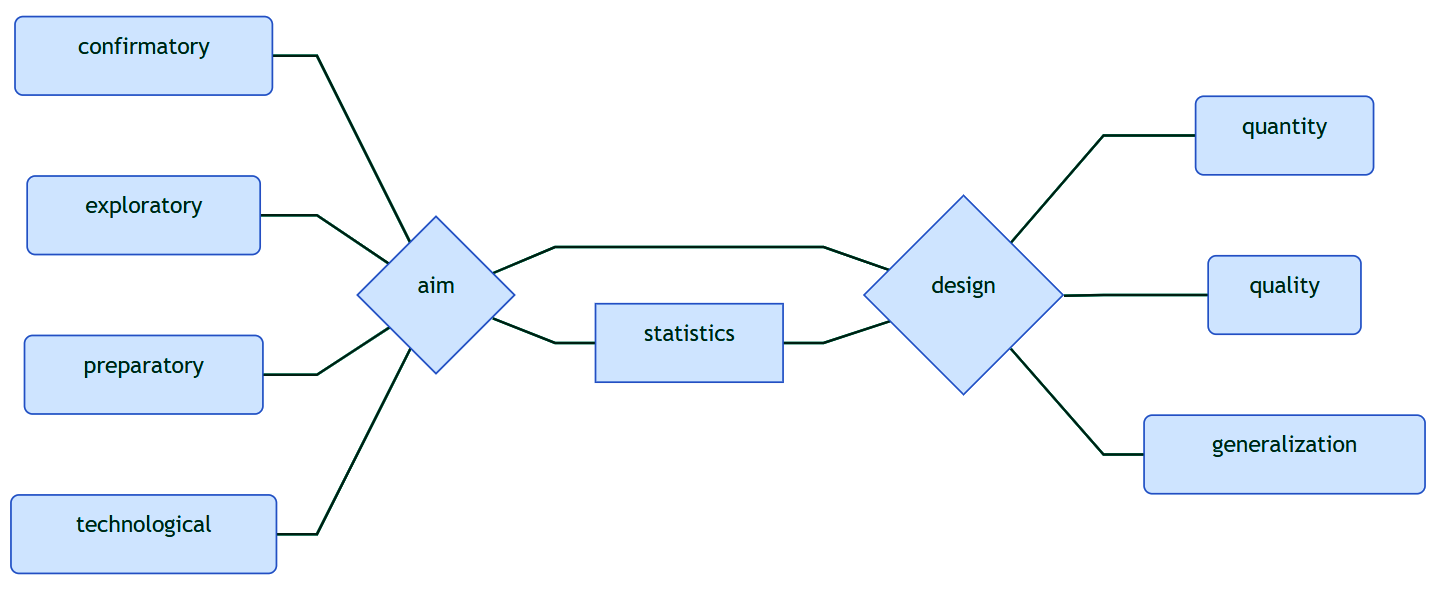
\includegraphics[width=0.75\textwidth,height=\textheight]{diagrammeR.png}
\caption{outline: key ingredients and main components}
\end{figure}

\newpage

\hypertarget{research-aim-first-key-ingredient}{%
\subsection{03 Research Aim: first key
ingredient}\label{research-aim-first-key-ingredient}}

\begin{itemize}
\tightlist
\item
  research aim: concisely express what the study intends to achieve

  \begin{itemize}
  \tightlist
  \item
    frame in terms of the essence, avoid unnecessary (technical) details
  \item
    be specific, go beyond very general statements
  \item
    operationalize, relate to empirical evidence \\
  \end{itemize}
\item
  focus, highlight research questions of primary interest

  \begin{itemize}
  \tightlist
  \item
    argue what the results should be -at a minimum- for it to be a
    successful study
  \item
    comment on additional gains the study could offer \\
  \end{itemize}
\item
  example: The aim is to show that the new treatment P is not worse than
  the common treatment Q, and we consider our study a success when the
  average score on measurement Y, with values expected between 16 and
  64, is maximally 10\% less for P. It will further be explored to what
  extent patient characteristics X could further explain the scores Y in
  both treatments.

  \begin{itemize}
  \tightlist
  \item
    detailed statement instead of `investigate' treatment
  \item
    linked to the empirical evidence
  \item
    focus, not a vague list of measurements
  \end{itemize}
\end{itemize}

\hypertarget{categorizations-of-research-aims}{%
\subsubsection{04 Categorizations of Research
Aims}\label{categorizations-of-research-aims}}

\begin{itemize}
\tightlist
\item
  the type of research aim determines how to deal with it (properties
  and requirements)
\item
  various categorizations can be considered, for example:

  \begin{itemize}
  \tightlist
  \item
    confirmatory / exploratory / preparatory / technological
  \item
    quantitative / qualitative
  \item
    inferential / descriptive \\
  \end{itemize}
\item
  note: type labels are informal, to be used for guidance only
\item
  typically, studies tend to be valued more if

  \begin{itemize}
  \tightlist
  \item
    they build on an understanding of future results (without being
    certain)
  \item
    they offer an future understanding beyond the study (wider / deeper)
  \item
    thus: if you can, frame it as such
  \end{itemize}
\end{itemize}

\hypertarget{descriptive-versus-inferential-research}{%
\paragraph{05 Descriptive versus Inferential
Research}\label{descriptive-versus-inferential-research}}

\begin{itemize}
\tightlist
\item
  inferential, study a population using a sample, implies generalization

  \begin{itemize}
  \tightlist
  \item
    (ideally) uses representative samples, large enough, randomly
    sampled
  \item
    more ambitious, thus difficult → guarantee inference is possible

    \begin{itemize}
    \tightlist
    \item
      relates to statistical testing, estimation, prediction
    \end{itemize}
  \end{itemize}
\item
  descriptive, study the observed data as such, no generalization

  \begin{itemize}
  \tightlist
  \item
    present data -as is- without reference to uncertainty nor p-values
  \item
    easy to perform → argue that data in itself is of interest

    \begin{itemize}
    \tightlist
    \item
      relates to summaries (average, median, \ldots, correlation) and
      values
    \end{itemize}
  \end{itemize}
\item
  note: inferential studies typically imply descriptive preliminary
  analysis
\end{itemize}

\hypertarget{quantitative-versus-qualitative-research}{%
\paragraph{06 Quantitative versus Qualitative
Research}\label{quantitative-versus-qualitative-research}}

\begin{itemize}
\tightlist
\item
  quantitative research addresses quantifiable empirical aspects

  \begin{itemize}
  \tightlist
  \item
    typically makes use of visualization and statistics to summarize and
    generalize
  \item
    can be descriptive and/or inferential
  \item
    typically aims to reduce complexity (operationalization before data
    analysis)
  \item
    main focus is summarizing and generalization → determines how to
    argues for it
  \end{itemize}
\item
  qualitative research addresses understanding

  \begin{itemize}
  \tightlist
  \item
    especially focused on reasons, opinions, motivations, \ldots{}
  \item
    is descriptive and can be hypothesis generating (inductive)
  \item
    typically embraces complexity
  \item
    main focus is interpretation / understanding \textasciitilde{}
    meaning → determines how to argues for it
  \end{itemize}
\item
  mixed methods combines both
\item
  rarely pure one or other
\item
  note: leaving out statistics does not make it a qualitative study
\item
  note: asking respondents questions does not make it qualitative
\end{itemize}

\hypertarget{objectives-confirmatory-explanatory-preparatory-technological}{%
\paragraph{07 Objectives: confirmatory, explanatory, preparatory,
techn(olog)ical}\label{objectives-confirmatory-explanatory-preparatory-technological}}

\hypertarget{confirmatory-research-aims}{%
\subparagraph{08 Confirmatory Research
Aims}\label{confirmatory-research-aims}}

\begin{itemize}
\tightlist
\item
  goal:: confirm an expected difference, relation, \ldots{}
\item
  means:: in advance specify results -at a minimum- to support claim

  \begin{itemize}
  \tightlist
  \item
    aim for

    \begin{itemize}
    \tightlist
    \item
      significant difference (superiority / non-inferiority) →
      statistical test
    \item
      equivalence given a margin of error → statistical test

      \begin{itemize}
      \tightlist
      \item
        absence of evidence is not evidence of absence
      \end{itemize}
    \item
      accurate estimate → statistical estimation
    \item
      expected observations → falsifying alternative hypotheses
    \item
      \ldots{} \\
    \end{itemize}
  \end{itemize}
\item
  focus::

  \begin{itemize}
  \tightlist
  \item
    explain (statistical) link research design and (especially) primary
    aim
  \item
    for a statistical test or estimation → calculate sample size using
    standard error

    \begin{itemize}
    \tightlist
    \item
      make assumptions and conditions explicit: effect size, statistics,
      type I and II errors
    \item
      conclude on required sample size: costs \& availability
    \end{itemize}
  \end{itemize}
\end{itemize}

\hypertarget{exploratory-research-aims}{%
\subparagraph{09 Exploratory Research
Aims}\label{exploratory-research-aims}}

\begin{itemize}
\tightlist
\item
  goal:: explore observations, possible differences, relations, \ldots{}

  \begin{itemize}
  \tightlist
  \item
    without any guarantee on what will be the results
  \end{itemize}
\item
  means:: in advance specify results -at a minimum- to support merit (no
  reference to significance or accuracy)

  \begin{itemize}
  \tightlist
  \item
    interest in data as such (descriptive)

    \begin{itemize}
    \tightlist
    \item
      no -primary- interest in statistical testing or estimation
    \end{itemize}
  \item
    interest in parameter estimates (differences, relations, \ldots)

    \begin{itemize}
    \tightlist
    \item
      aim for statistical testing or estimation but

      \begin{itemize}
      \tightlist
      \item
        no guarantee sufficient power and/or accuracy
      \item
        maybe try `upgrading' it to confirmatory research ? → decide on
        effect of interest
      \end{itemize}
    \end{itemize}
  \item
    interest in prediction

    \begin{itemize}
    \tightlist
    \item
      aim for cross-validation (does not include standard errors)

      \begin{itemize}
      \tightlist
      \item
        open question how to argue sample size, refer to similar
        research / common practice
      \item
        possible to justify afterwards using bootstrapping → discuss
        criteria
      \end{itemize}
    \end{itemize}
  \item
    qualitative research \\
  \end{itemize}
\item
  focus::

  \begin{itemize}
  \tightlist
  \item
    argue why the data or parameter estimates by themselves are of
    interest

    \begin{itemize}
    \tightlist
    \item
      even if not significant/inaccurate
    \item
      or why significance/accuracy is likely

      \begin{itemize}
      \tightlist
      \item
        based on similar existing research
      \end{itemize}
    \item
      put more weight on substantive arguments
    \end{itemize}
  \item
    sample size -justification- with balance information and cost

    \begin{itemize}
    \tightlist
    \item
      argue that merit outweighs cost
    \item
      low cost of collection, or data already available (eg.,
      retrospective)
    \end{itemize}
  \item
    still explain (statistical) link research design and potential
    inferences
  \end{itemize}
\end{itemize}

\hypertarget{preparatory-research-aims}{%
\subparagraph{10 Preparatory Research
Aims}\label{preparatory-research-aims}}

\begin{itemize}
\tightlist
\item
  goal:: prepare for a future study\ldots{} typically a small scale
  set-up
\item
  means:: in advance specify what information is required for a future
  study and how it will be obtained

  \begin{itemize}
  \tightlist
  \item
    pilot study

    \begin{itemize}
    \tightlist
    \item
      aim to successfully set up future study
    \end{itemize}
  \item
    phase I and II clinical designs

    \begin{itemize}
    \tightlist
    \item
      aim to avoid risk, harm, \ldots{} future study
    \item
      requires decision criteria to proceed or not
    \end{itemize}
  \item
    database development, data collection procedures, \ldots{} \\
  \end{itemize}
\item
  focus::

  \begin{itemize}
  \tightlist
  \item
    argue based on information required for future (actual) study

    \begin{itemize}
    \tightlist
    \item
      explain how unavailable information is obtained
    \item
      argument could be (partially) qualitative, descriptive, \ldots{}

      \begin{itemize}
      \tightlist
      \item
        example: understand instructions, register observations,
        \ldots{}
      \end{itemize}
    \end{itemize}
  \item
    results are not by themselves of interest

    \begin{itemize}
    \tightlist
    \item
      no statistical testing is implied, that is for future (actual)
      studies
    \end{itemize}
  \item
    sample size -justification- based on an absolute minimal cost

    \begin{itemize}
    \tightlist
    \item
      for example, with animal experiments typically 3 animals per
      condition

      \begin{itemize}
      \tightlist
      \item
        allow the estimation of variance
      \end{itemize}
    \item
      low cost of collection, or data already available (eg.,
      retrospective)
    \end{itemize}
  \end{itemize}
\end{itemize}

\hypertarget{technological-advancements}{%
\subparagraph{11 Techn(olog)ical
advancements}\label{technological-advancements}}

\begin{itemize}
\tightlist
\item
  goal:: to design, engineer, create, \ldots{} not to extract
  information from the outside world
\item
  means:: argue merit of the final product, rarely any statistics
  involved
\item
  focus::

  \begin{itemize}
  \tightlist
  \item
    argument based on what the advancement offers, in balance with the
    costs
  \item
    no statistical justification, and that is alright !!
  \end{itemize}
\end{itemize}

\hypertarget{research-design-second-key-ingredient}{%
\subsection{12 Research Design: second key
ingredient}\label{research-design-second-key-ingredient}}

\begin{itemize}
\tightlist
\item
  research design: strategy to achieve the research aim

  \begin{itemize}
  \tightlist
  \item
    effective (question can be answered) and efficient (with
    acceptable/minimal costs)
  \item
    determines how (potential) observations provide information on
    research aim

    \begin{itemize}
    \tightlist
    \item
      a poor design makes a study inefficient at best, completely
      ineffective at worst
    \item
      statistics can not solve design problems
    \item
      example: study different treatment effects with fixed order
      \textasciitilde{} confounding\\
      ~\\
    \end{itemize}
  \end{itemize}
\item
  three types of design attributes

  \begin{itemize}
  \tightlist
  \item
    quantity of observations (sample size)
  \item
    quality of observations, dependent on

    \begin{itemize}
    \tightlist
    \item
      what is observed
    \item
      how it is observed (method)
    \item
      under which conditions it is observed (\textasciitilde{}
      variables)
    \end{itemize}
  \item
    generalizability (from sample to population), dependent on

    \begin{itemize}
    \tightlist
    \item
      selection/allocation of research units
    \item
      missing data mechanism\\
    \end{itemize}
  \end{itemize}
\item
  focus, highlight the good choices when relevant

  \begin{itemize}
  \tightlist
  \item
    show what is done right, that you have it under control
  \item
    discuss in relation to relevance, maybe name-drop
  \item
    do not dwell on what you (may) fail to deal with\\
  \end{itemize}
\end{itemize}

\hypertarget{quantity-of-observations}{%
\subsubsection{13 Quantity of
Observations}\label{quantity-of-observations}}

\begin{itemize}
\tightlist
\item
  collect enough relevant observations

  \begin{itemize}
  \tightlist
  \item
    more observations are more informative, ensure that sufficient
    (effective)

    \begin{itemize}
    \tightlist
    \item
      more observations required if they are less informative by
      themselves (see quality)
    \end{itemize}
  \item
    more observations may be more costly, ensure not too many
    (efficient)

    \begin{itemize}
    \tightlist
    \item
      remember, costs in terms of time, money, risk, stress, \ldots{} \\
    \end{itemize}
  \end{itemize}
\item
  justify quantity of observations

  \begin{itemize}
  \tightlist
  \item
    typically only required for the primary research questions, and/or
    costly observations
  \item
    for confirmatory research, perform sample size -calculation-

    \begin{itemize}
    \tightlist
    \item
      specify statistical test(s) or estimation(s) in focus (implied by
      what -at a minimum- ensures a successful study).
    \item
      specify effect size aimed for, justify both the effect and the
      uncertainty

      \begin{itemize}
      \tightlist
      \item
        effect: ideally justified substantively or at least referring to
        common practice or literature
      \item
        uncertainty: variance of measurement, ideally based on earlier
        data/research or pilot
      \item
        use rules of thumb when all reasoning fails, only
      \end{itemize}
    \item
      specify operational characteristics (type I error \(\alpha\) and
      type II error \(\beta\) are related)

      \begin{itemize}
      \tightlist
      \item
        note: an \(\alpha\) of .05 and power of .8 (\(\beta\) = .2)
        implies type I error 4 times more severe
      \end{itemize}
    \end{itemize}
  \item
    for exploratory / preparatory research this includes a sample size
    -justification-

    \begin{itemize}
    \tightlist
    \item
      feasibility and/or low cost
    \item
      minimum requirement for a first impression
    \item
      similar / equivalent research
    \end{itemize}
  \end{itemize}
\end{itemize}

\hypertarget{quality-of-observations}{%
\subsubsection{14 Quality of
Observations}\label{quality-of-observations}}

\begin{itemize}
\tightlist
\item
  collect informative observations (especially important if relatively
  few)

  \begin{itemize}
  \tightlist
  \item
    observations made with most informative method

    \begin{itemize}
    \tightlist
    \item
      validity \& reliability
    \item
      example stress:

      \begin{itemize}
      \tightlist
      \item
        self rating vs.~neuro-endocrine vs.~\ldots{}
      \item
        memory vs.~now vs.~imagined situation vs.~\ldots{}
      \end{itemize}
    \end{itemize}
  \item
    observations made under the most informative conditions

    \begin{itemize}
    \tightlist
    \item
      link with research question
    \item
      include suspected confounders
    \item
      example stress:

      \begin{itemize}
      \tightlist
      \item
        short/long term difference - evolution
      \item
        lab - naturalistic ? \\
      \end{itemize}
    \end{itemize}
  \end{itemize}
\item
  general principle: isolate the effect, avoid / measure unwanted
  influences

  \begin{itemize}
  \tightlist
  \item
    control confounding variables (\textasciitilde{} complete the model)
  \item
    maximize systematic variability (\textasciitilde{} explained
    variance)
  \item
    minimize non-systematic variability (\textasciitilde{} unexplained
    variance) \\
  \end{itemize}
\item
  highlight how quality is ensured, lack of quality is avoided

  \begin{itemize}
  \tightlist
  \item
    show you have it under control, you know why you set up your study
    this way
  \item
    be specific, relate to your research design and aim
  \item
    do not highlight weaknesses (too strongly)
  \end{itemize}
\end{itemize}

\hypertarget{quality-of-observations-confounders}{%
\subsubsection{15 Quality of Observations ---
Confounders}\label{quality-of-observations-confounders}}

\begin{itemize}
\tightlist
\item
  explain control of confounding (unwanted outside influence)

  \begin{itemize}
  \tightlist
  \item
    balance out confounding

    \begin{itemize}
    \tightlist
    \item
      randomization (large enough sample size)
    \item
      stratified randomization
    \end{itemize}
  \item
    measure confounding

    \begin{itemize}
    \tightlist
    \item
      repeated measures (\textasciitilde{} conditioning)
    \item
      cross-over designs (\textasciitilde{} conditioning)
    \item
      blocking, keep variances sources stable and estimate
      (\textasciitilde mini-experiments)
    \end{itemize}
  \item
    avoid confounding

    \begin{itemize}
    \tightlist
    \item
      matching, create similar groups to compare
    \item
      (double-) blinding, avoid influence experimenter/experimented
    \end{itemize}
  \item
    and more \ldots{} \\
  \end{itemize}
\item
  often more complex designs are more efficient but also more complex to
  analyze

  \begin{itemize}
  \tightlist
  \item
    eg., mixed models to deal with repeated measures
  \end{itemize}
\end{itemize}

\hypertarget{quality-of-observations-non-systematic-variability}{%
\subsubsection{16 Quality of Observations --- Non-Systematic
Variability}\label{quality-of-observations-non-systematic-variability}}

\begin{itemize}
\tightlist
\item
  variability that is not understood \textasciitilde{} uncertainty
\item
  explain minimization of non-systematic variability

  \begin{itemize}
  \tightlist
  \item
    use of proper measurement tools

    \begin{itemize}
    \tightlist
    \item
      ensure reliability / precision to avoid noisy measurements
    \item
      combine measurement tools
    \item
      repeat observations (replications) to average out noisy
      measurements
    \item
      use tools that are well understood/studied
    \end{itemize}
  \item
    use of all information available

    \begin{itemize}
    \tightlist
    \item
      include all relevant predictors

      \begin{itemize}
      \tightlist
      \item
        not only focus on main variables of interest (\textasciitilde{}
        model)
      \item
        potentially consider combinations (interaction, polynomial,
        \ldots)
      \end{itemize}
    \item
      avoid the use of categories when continuous registrations are
      available
    \item
      consider (multiple) imputation when missingness is modest
    \end{itemize}
  \end{itemize}
\end{itemize}

\hypertarget{quality-of-observations-systematic-variability}{%
\subsubsection{17 Quality of Observations --- Systematic
Variability}\label{quality-of-observations-systematic-variability}}

\begin{itemize}
\tightlist
\item
  variability that is understood \textasciitilde{} information
\item
  explain maximization of systematic variability

  \begin{itemize}
  \tightlist
  \item
    maximally differentiate conditions

    \begin{itemize}
    \tightlist
    \item
      DoE, design of experiments
    \item
      example: detect change, effectiveness, \ldots{}
    \end{itemize}
  \item
    largely implies minimization of non-systematic variability

    \begin{itemize}
    \tightlist
    \item
      \textasciitilde{} appropriate and sufficiently rich model for the
      observations
    \end{itemize}
  \end{itemize}
\end{itemize}

\hypertarget{quality-of-observations-experimental-control}{%
\subsubsection{18 Quality of Observations --- Experimental
Control}\label{quality-of-observations-experimental-control}}

\begin{itemize}
\tightlist
\item
  safeguard quality of information easier if (some) control on
  conditions

  \begin{itemize}
  \tightlist
  \item
    experimental study, exerts control by definition

    \begin{itemize}
    \tightlist
    \item
      choose the conditions of observation
    \item
      randomize the allocation to conditions
    \item
      necessary condition for causal conclusions
    \end{itemize}
  \item
    observational study, does not exert control, efficiency loss at best

    \begin{itemize}
    \tightlist
    \item
      increase quantity to compensate loss in quality
    \item
      includes naturalistic data collections, surveys, retrospective
      data collection, \ldots{} \\
    \end{itemize}
  \end{itemize}
\item
  highlight what you can control, and how you use that control
\end{itemize}

\hypertarget{generalizability}{%
\subsubsection{19 Generalizability}\label{generalizability}}

\begin{itemize}
\tightlist
\item
  collect a sample of observations with the aim to generalize
  (inference)

  \begin{itemize}
  \tightlist
  \item
    conclude upon more than just the observed sample → avoid biased
    sampling
  \item
    type of sampling

    \begin{itemize}
    \tightlist
    \item
      probabilistic (sampling: random, stratified, multi-stage, \ldots.)

      \begin{itemize}
      \tightlist
      \item
        necessary for conclusive, unbiased, objective inferences
      \item
        conclude upon population sampled from
      \end{itemize}
    \item
      non-probabilistic (sampling: diversity, expert, \ldots.)

      \begin{itemize}
      \tightlist
      \item
        potentially biasing, more subjective, and best used only
        exploratory, descriptive
      \item
        argue why not biasing in your case
      \item
        no issue for qualitative studies
      \end{itemize}
    \end{itemize}
  \end{itemize}
\item
  missing data: safeguard against / remediate

  \begin{itemize}
  \tightlist
  \item
    generalization fails when substantial non-random missing data

    \begin{itemize}
    \tightlist
    \item
      depends on mechanism of missingness

      \begin{itemize}
      \tightlist
      \item
        problem if not at random → biased
      \item
        results in loss of precision
      \end{itemize}
    \end{itemize}
  \item
    explain how it is avoided and dealt with

    \begin{itemize}
    \tightlist
    \item
      how many missing values to expect, for what reason
    \item
      what to do to further minimize this number

      \begin{itemize}
      \tightlist
      \item
        improve data collection
      \item
        obtain information to deal with missingness
      \end{itemize}
    \end{itemize}
  \end{itemize}
\end{itemize}

\hypertarget{statistics}{%
\subsection{20 Statistics}\label{statistics}}

\begin{itemize}
\tightlist
\item
  link between research design and research aim

  \begin{itemize}
  \tightlist
  \item
    highlight how given a design, statistics is able to resolve the aims

    \begin{itemize}
    \tightlist
    \item
      focus on primary research questions
    \item
      sketch of secondary research questions → maybe do some
      name-dropping
    \end{itemize}
  \item
    reflect on the type of data and challenges they offer

    \begin{itemize}
    \tightlist
    \item
      continuous/ordinal/nominal
    \item
      skewed, outliers, boundary values, \ldots{}
    \item
      but avoid being vague or to give a lecture statistics 101
    \end{itemize}
  \end{itemize}
\item
  introduce intended statistical analysis

  \begin{itemize}
  \tightlist
  \item
    include

    \begin{itemize}
    \tightlist
    \item
      statistical tests (evaluate whether effects exist; p-values)
    \item
      statistical estimation (evaluate confidence interval)
    \item
      prediction (evaluate model fit using individual observations)
    \end{itemize}
  \item
    specify the expected inferences, be specific
  \end{itemize}
\item
  note: sample size calculations are not part of statistics

  \begin{itemize}
  \tightlist
  \item
    often based on simplified statistical testing/estimation
  \item
    typically not discussed separately
  \end{itemize}
\end{itemize}

\hypertarget{small-example}{%
\subsubsection{21 Small Example}\label{small-example}}

The aim is to show that the proposed treatment is an improvement over
the current standard method, as it will show in higher scores on my
measurement.

Participants are randomized to either the treatment or control group.
The control group is given a dummy treatment of which a post experiment
survey addresses whether participants were aware. Each participant is
measured twice, once immediately before and once immediately after the
(dummy) treatment was administered. Each measurement results in a
continuous score on a 0-10 scale. A mixed model compares the change
between post and pre treatment measurement while accounting for
pre-treatment scores. Also the following possible confounders will be
included: \ldots{}

A sample size was derived for a t-test that focuses on the detection of
a post-treatment difference of 2 in favor of the treatment. The minimal
clinical difference was decided upon by our expert panel. In literature,
the standard method is indicated to have a population standard deviation
of about 4. Because no information is available on the new treatment it
is assumed that the same population standard deviation applies. This
leads to a sample size of 51 patients in each of both groups, required
for a one-sided test, type I error of .05 and power of .8. Earlier
experiments showed a drop-out of about 10\%, so 51 * (100/(100-10))
\textless{} 57 patients are included per group. Because the more
advanced statistical test and the inclusion of various potential
confounders, this number can be considered conservative but realistic.
This number will also present no difficulties to collect in our center.

\hypertarget{some-practical-suggestions}{%
\subsection{22 Some Practical
Suggestions}\label{some-practical-suggestions}}

\begin{itemize}
\item
  isolate methodological / statistical arguments from substantive
  reasoning
\item
  use concise and consistent labeling of data and conditions
\item
  visualize and structure wherever possible

  \begin{itemize}
  \item
    data collection process
  \item
    categories of observations and their relation
  \item
    a text a statistical referee does not want to read

    We will compare the effect of {[}treatment{]} on {[}condition{]} by
    randomizing mice over groups with {[}description of procedure the
    statistician does not need to know about{]} and groups with
    {[}description of another procedure the statistician does not need
    to know about {]}. Each procedure will be performed with 2
    {[}substances{]} and each at 3 different doses, namely
    {[}dosages{]}.\\
    We expect procedure A with substance 1, respectively substance 2 to
    achieve on average 13 units, respectively 15 units and a standard
    deviation of 1, respectively 1.5 at the lowest dosis, with a 10\%
    increase in both mean and standard deviation at the second dosis and
    20\% increase for the third. For procedure B with substance 1,
    respectively substance 2 to achieve on average 11 units,
    respectively 13 units and a standard deviation of 1, respectively
    1.3 at the lowest dosis, with a 10\% increase in both mean and
    standard deviation at the second dosis and 20\% increase for the
    third. We will also include a control group which achieves an
    average of 6 and standard deviation 0.5, where we expect dosis to
    have no effect.
  \item
    could be turned into

    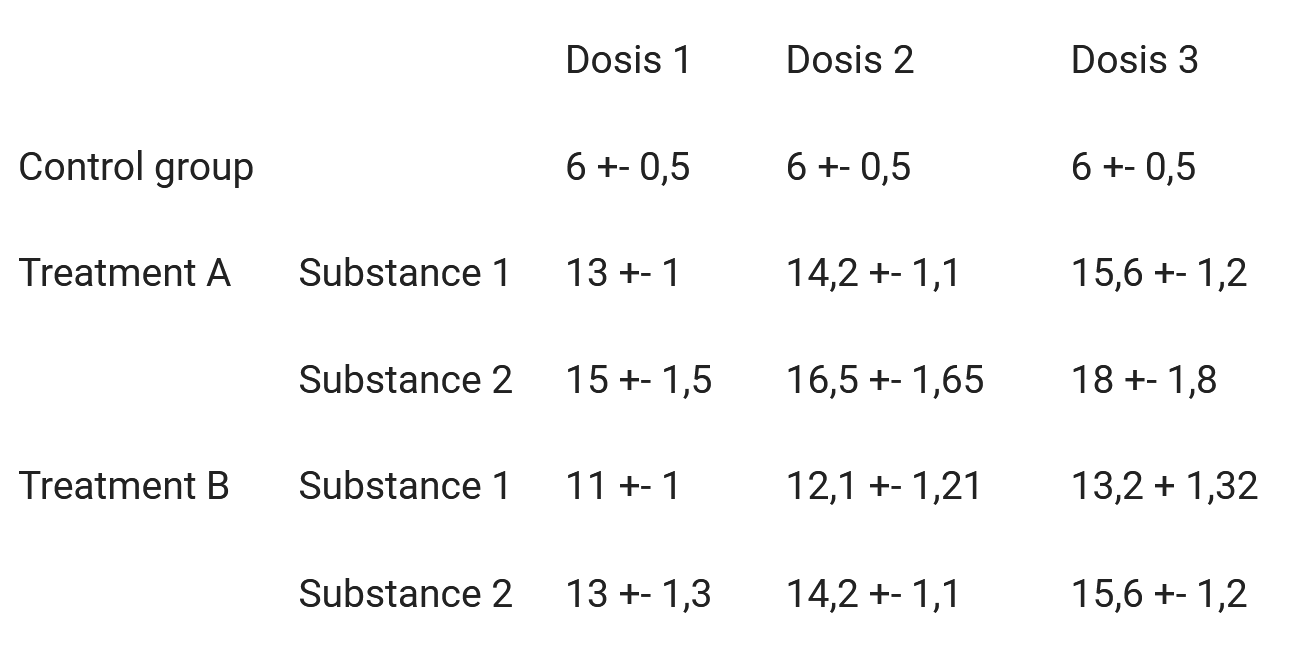
\includegraphics[width=0.7\textwidth,height=\textheight]{tableECD.png}
  \item
    experiments can also be visualized, eg., time-line

    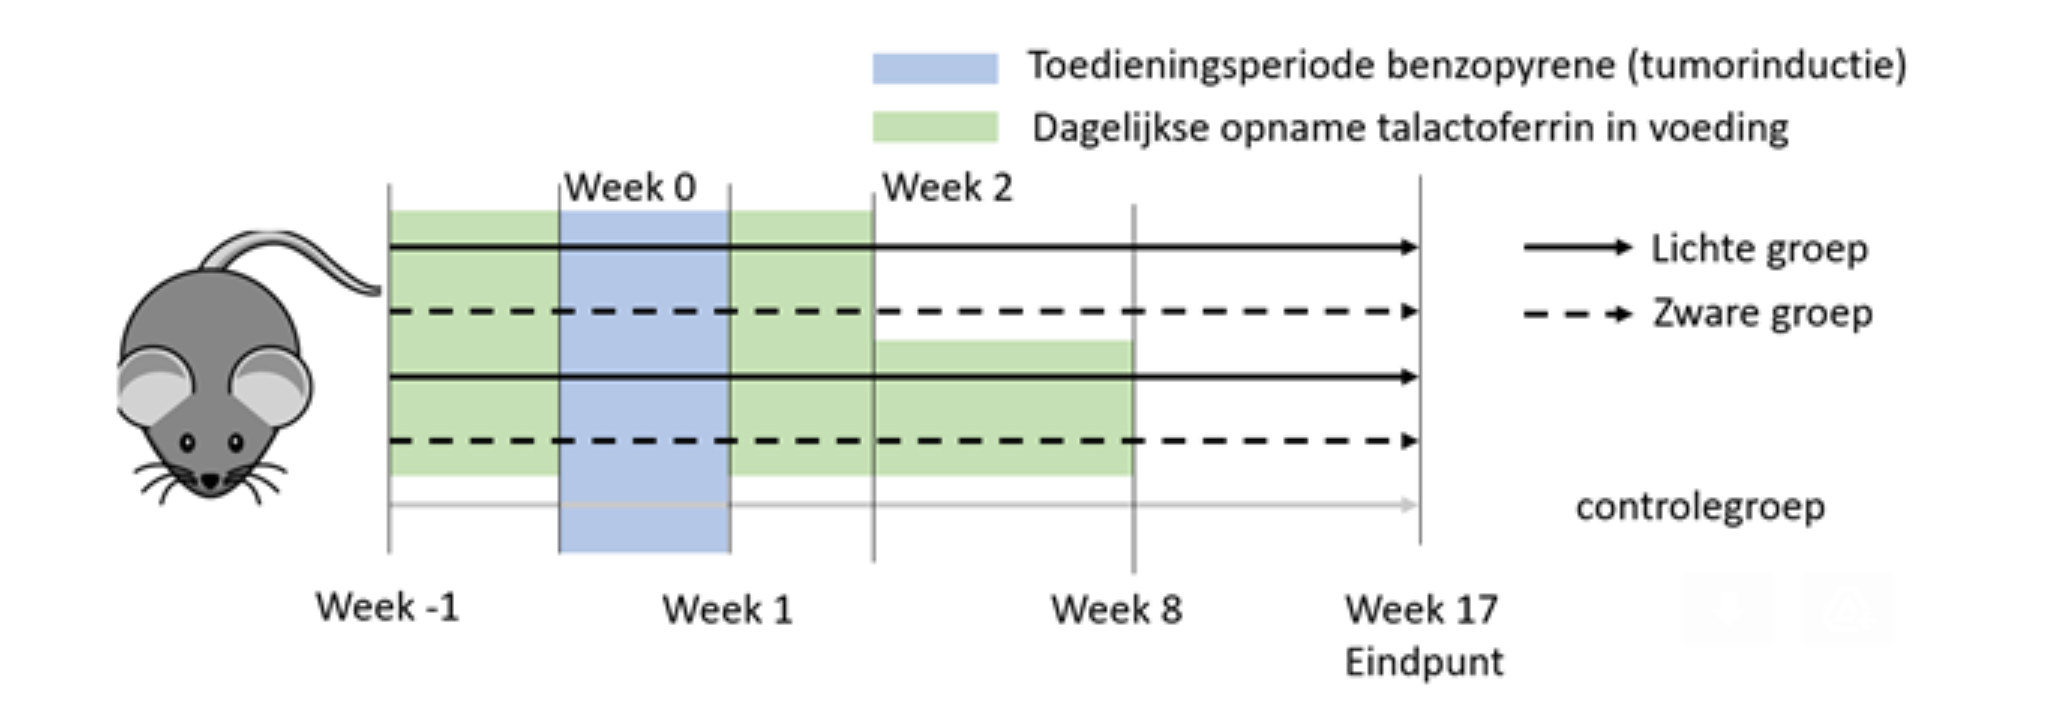
\includegraphics{figECD.png}
  \item
    design: tables to list conditions between (rows) and within
    (columns)

    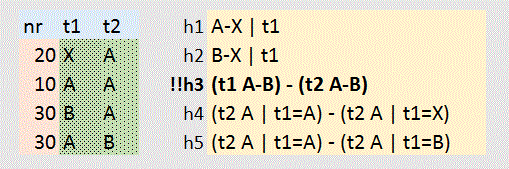
\includegraphics{conds.png}
  \end{itemize}
\end{itemize}

\newpage

\hypertarget{conclusion}{%
\subsection{23 Conclusion}\label{conclusion}}

\begin{itemize}
\tightlist
\item
  be clear on your aim and how to reach it with an appropriate design
\item
  highlight what is essential for your type of study
\item
  highlight the good choices that you have made
\item
  focus on what deserves focus
\item
  use a language understood by the relevant referee

  \begin{itemize}
  \tightlist
  \item
    statistical lingo
  \item
    visualization / structure
  \end{itemize}
\end{itemize}

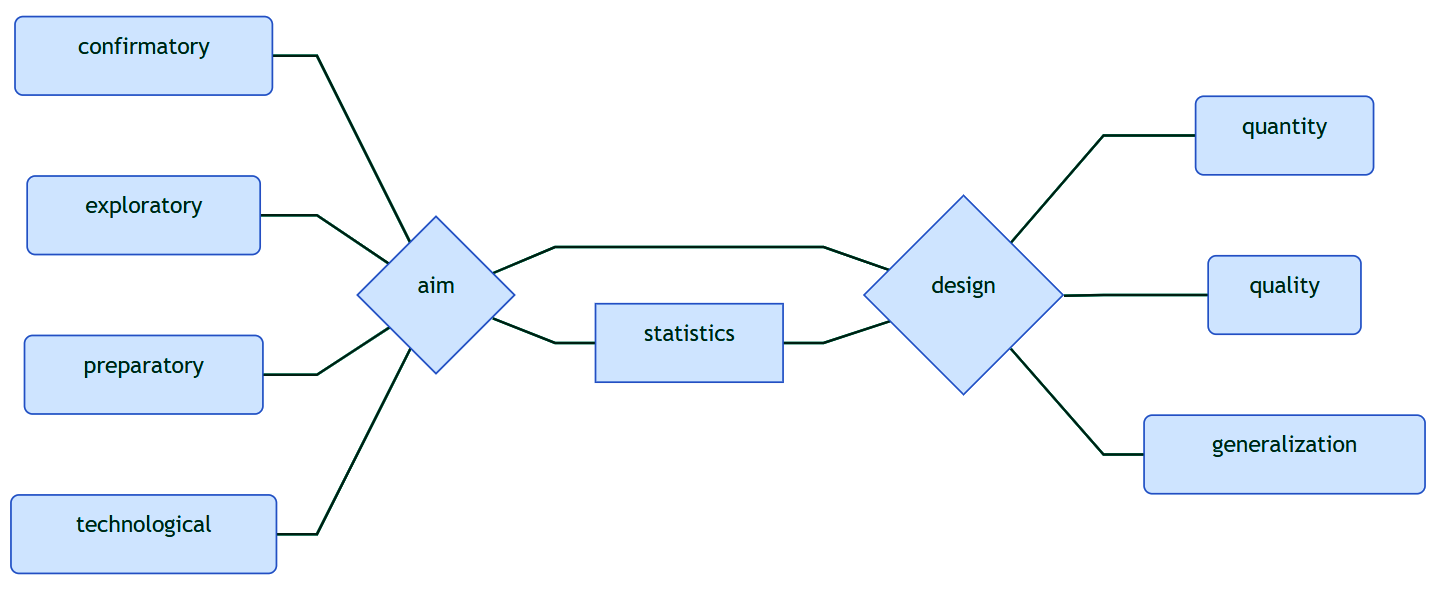
\includegraphics[width=0.7\textwidth,height=\textheight]{diagrammeR.png}

\newpage

\hypertarget{section}{%
\section[ ]{\texorpdfstring{
\protect
\includegraphics[width=0.4\textwidth,height=\textheight]{icds.png}}{ }}\label{section}}

Methodological and statistical support to help make a difference

\begin{itemize}
\item
  ICDS provides complementary support in methodology and statistics to
  our research community, for both individual researchers and research
  groups, in order to get the best out of them
\item
  ICDS aims to address all questions related to quantitative research,
  and to further enhance the quality of both the research and how it is
  communicated
\end{itemize}

website: \url{https://www.icds.be/} includes information on who we
serve, and how

booking: \url{https://www.icds.be/consulting/} for individual
consultations

\end{document}
